%# -*- coding: utf-8-unix -*-
%%==================================================
\chapter{java基础}
\label{chap1}
\begin{itemize}[noitemsep,topsep=0pt,parsep=0pt,partopsep=0pt]
	\item ...
\end{itemize}

\section{知识点和方法论}

\subsection{知识点}
\subsubsection{双亲委派机制}
Bootstrap classLoader:主要负责加载核心的类库(java.lang.*等),构造ExtClassLoader和APPClassLoader。

ExtClassLoader:主要负责加载jre/lib/ext目录下的一些扩展的jar。

AppClassLoader:主要负责加载应用程序的主函数类

好处

如果有人想替换系统级别的类:String.java。篡改它的实现,在这种机制下这些系统的类已经被Bootstrap classLoader加载过了(为什么?因为当一个类需要加载的时候,最先去尝试加载的就是BootstrapClassLoader),所以其他类加载器并没有机会再去加载,从一定程度上防止了危险代码的植入。

\begin{figure}
	\centering
	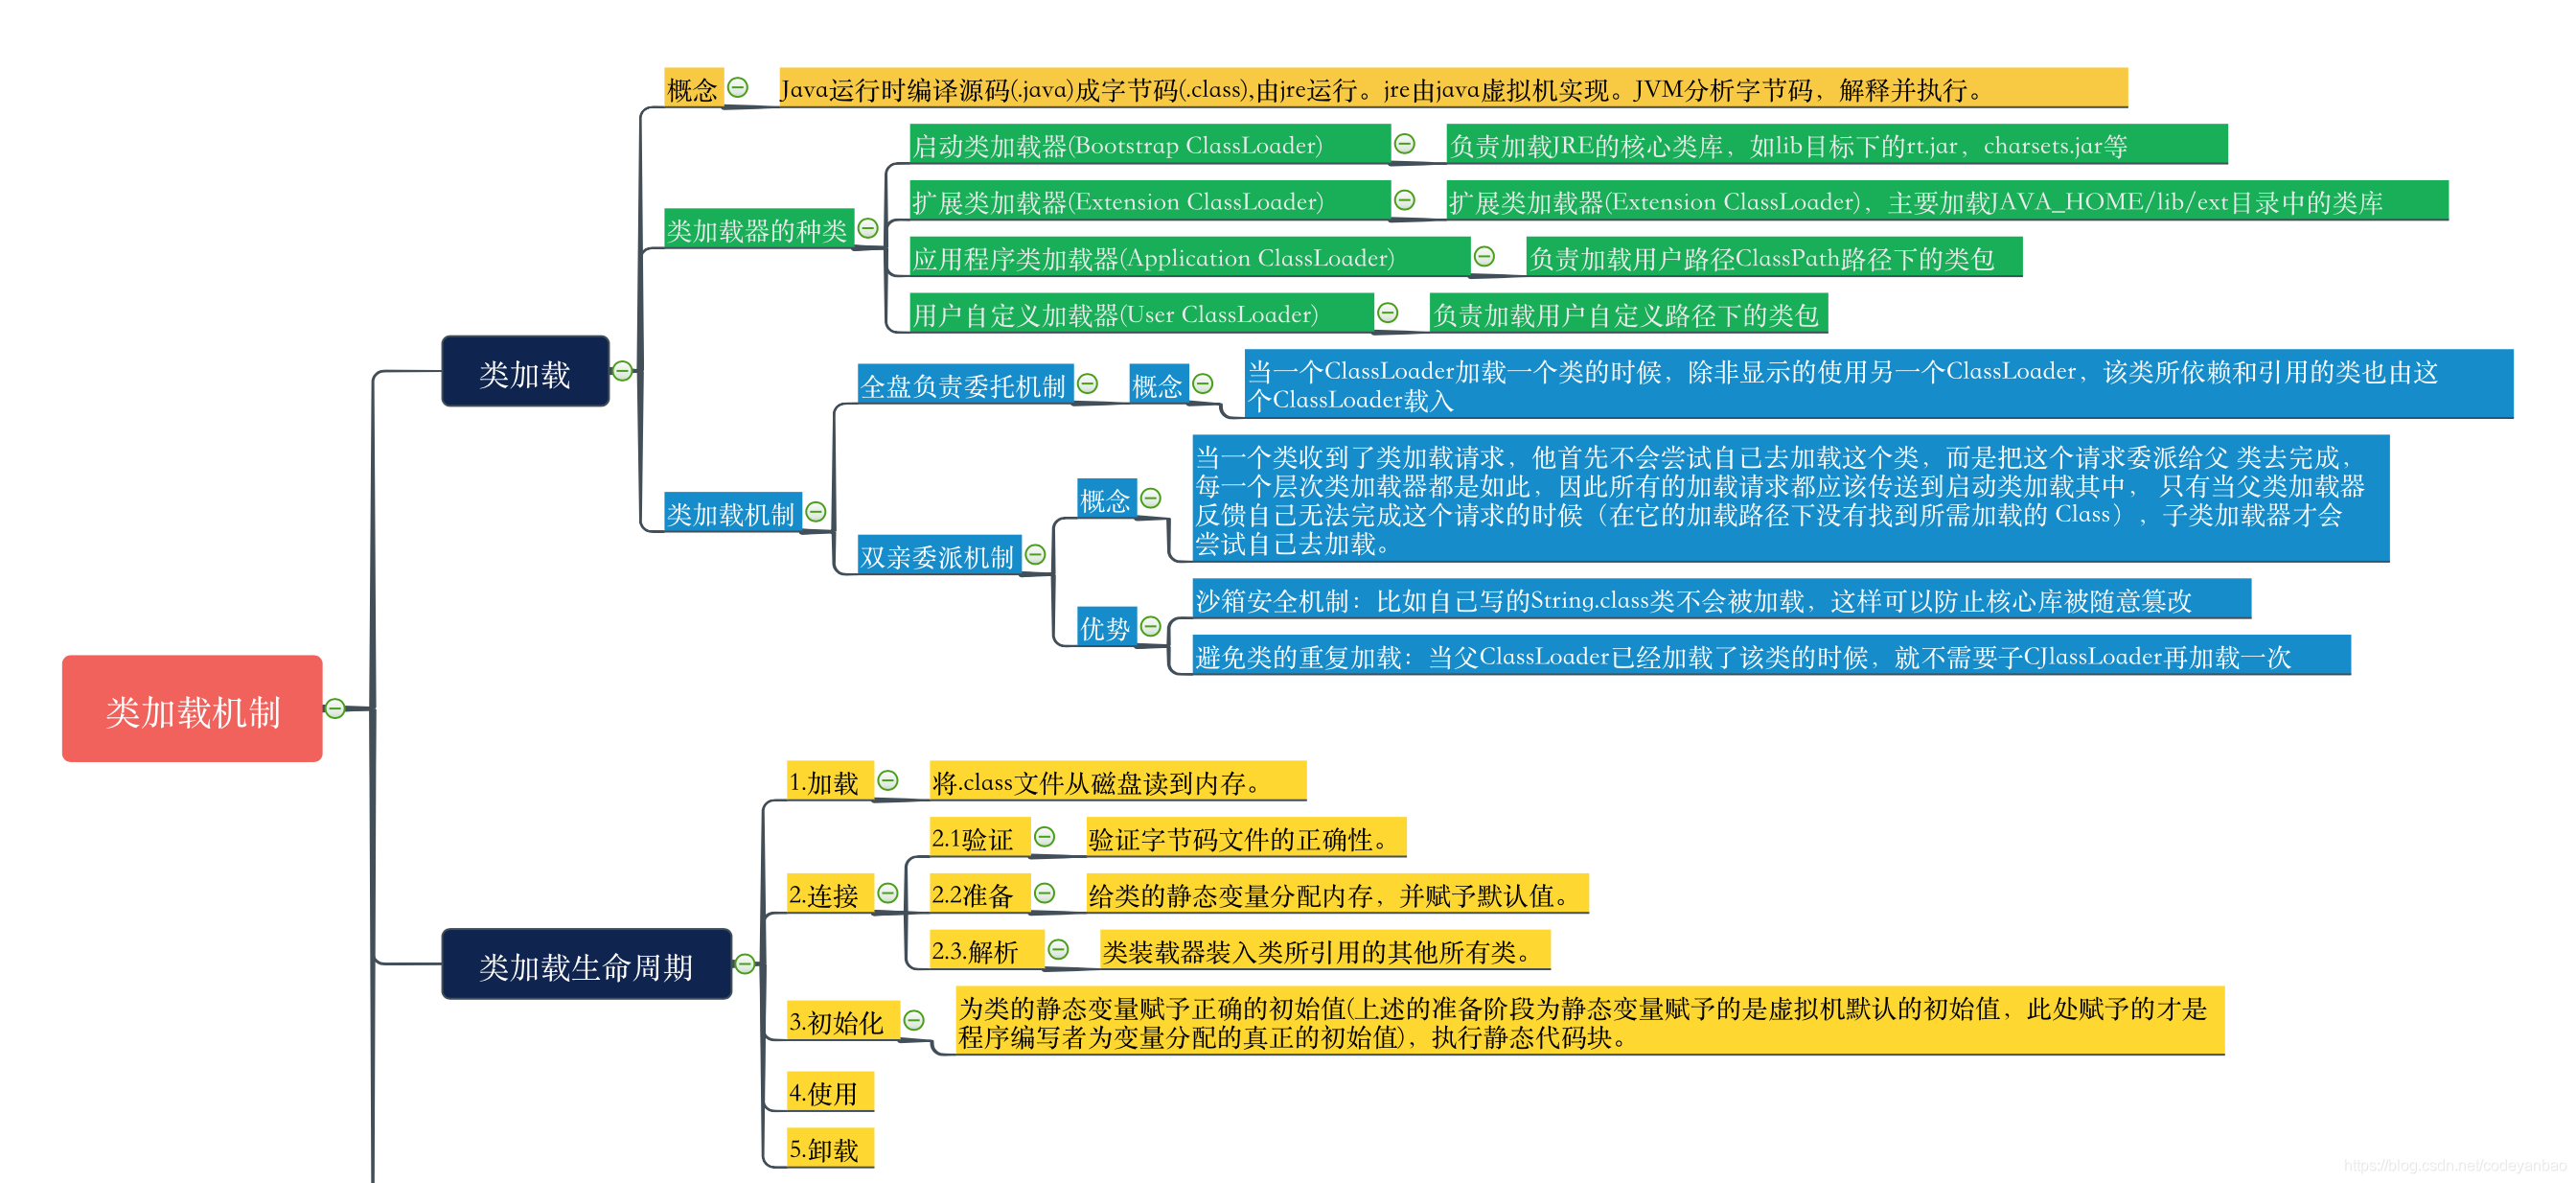
\includegraphics[width=1\linewidth]{figures/shuangqin.png}
	\caption{shuangqin}
	\label{fig:shuangqin}
\end{figure}


\subsubsection{AQS 浅析}
简单而言就是一个并发包组件, ReentrantLock 在其之上构建的.

AQS 全称: AbstractQueuedSynchronizer 抽象队列同步器

里面state=0 表示没有线程占用这个资源, 还有一个对加锁线程的记录. 当没有获得资源的线程就会进入等待队列,直到获取资源的线程自己释放了资源. 队列中第二个线程就会被唤醒.

\subsubsection{java加密算法浅析}

MD5是不可逆加密,不可以用来加密文本,DES和RC4是对称加密,RSA是不对称加密,都可以用于文本加密
\subsubsection{java 使用流的方式去除某些变量}
$$
	List<String> ss = list.stream().filter(element->null!=element).collect(Collectors.toList());
$$
\subsubsection{java中的变量如果直接赋值为null下面直接使用的话, 会报空指针异常}


\subsubsection{java接口中默认成员变量的修饰符}

public static final int 静态最终变量.

public abstract  抽象方法

\subsubsection{快速排序}
参照图解
\url{https://blog.csdn.net/pengzonglu7292/article/details/84938910}

简单的来说就是双指针交汇运动.




\subsubsection{UML图标}

\url{https://blog.csdn.net/u011125703/article/details/50935322}

泛华, 依赖, 关联, 聚合, 实现 和 组合

空心菱形是聚合

实心菱形是组合

一条直线是关联


\subsubsection{session与token的区别?}
简单来说session是以sessionid - 和 session 存储的. sessionid存储在cookie中. 每次请求会带上.
token 简单来说就是一串能表示用户身份的随机字符串. 其实功能和sessionid差不多.
\subsubsection{注解以及相关问题}
注解的使用其实是一个接口继承了annotation接口, 使用@interface 来定义一个注解

一般通过反射来读取注解

有类注解, 属性注解 和 方法注解.

@Retention(value = RetentionPolicy.RUNTIME) 是运行时可见的注解

可以定义@Target(value= {ElementType.TYPE,ElementType.METHOD,ElementType.FIELD})  是定义注解的组成

getAnnotation(MyAnnotationDefinition.class); 获取类注解

clazz.getDeclaredMethods(); 获取方法注解

Field nameField =  clazz.getDeclaredField("name"); 获取属性注解


\subsubsection{juc arraylist \& int}
static AtomicInteger atomicInteger = new AtomicInteger(0);

atomicInteger.getAndIncrement();

基于CAS

CopyOnWriteArrayList c = new CopyOnWriteArrayList();

c.add(2);

CopyOnWriteArrayList这是一个ArrayList的线程安全的变体,其原理大概可以通俗的理解为:初始化的时候只有一个容器,很长一段时间,这个容器数据、数量等没有发生变化的时候,大家(多个线程),都是读取(假设这段时间里只发生读取的操作)同一个容器中的数据,所以这样大家读到的数据都是唯一、一致、安全的,但是后来有人往里面增加了一个数据,这个时候CopyOnWriteArrayList 底层实现添加的原理是先copy出一个容器(可以简称副本),再往新的容器里添加这个新的数据,最后把新的容器的引用地址赋值给了之前那个旧的的容器地址,但是在添加这个数据的期间,其他线程如果要去读取数据,仍然是读取到旧的容器里的数据。

使用可重入锁进行数组的锁定

\begin{lstlisting}
public boolean add(E e) {
	final ReentrantLock lock = this.lock;
	lock.lock();
	try {
		Object[] elements = getArray();
		int len = elements.length;
		Object[] newElements = Arrays.copyOf(elements, len + 1);
		newElements[len] = e;
		setArray(newElements);
		return true;
	} finally {
		lock.unlock();
	}
}
\end{lstlisting}
\subsubsection{本地方法栈溢出的情况}
创建了过多的线程, 线程独立, 请求虚拟机栈和本地方法栈 -- Stack Overflow

\subsubsection{堆内存溢出}
oom out of memory

申请的动态数据占据了过多的内存


\subsubsection{HTTP请求头中有什么参数}
请求报文


1. 请求方法 GET? POST

2. HTTP版本 1.1 2 3??

3. accept 期望接收的语言 zh en ??

4. user-agent: 访问者是通过什么工具来请求的

5. cache-control 是否强制刷新


相应报文

1. 状态码 200

2. 响应体 一般是json 数据

3. content-type: 响应体里面的数据类型  image之类的
\subsubsection{HTTP请求资源的方式}
GET: 获取资源

POST: 创建资源

PUT: 创建(更新资源)

DELETE: 删除资源
\subsubsection{如何防止SQL注入}
使用预编译的方法来, 比如PrepareStatement类下面的setString方法来对参数进行处理, 简单来说
\subsubsection{如何实现10000个qq判断是否在线的情况}
java 中有BitSet这个类, 然后使用这个类来实现判断是否在线的情况 \par
\subsubsection{hashmap死锁产生情况}
1.7 版本的死锁是在 rehash方法中的transfer方法产生的, 因为在扩容的过程中, 主要关于两个指针, e指针指向当前节点, next是e的下一个指针, 因为采用头插法会前后顺序调换, 导致产生换的现象. \par
\subsubsection{谈谈对ConcurrentHashMap的扩容机制}
1.7版本: \par
1. 1.7版本的ConcurrentHashmap是基于Segment分段实现的\par
*. Segment 依赖 ReentrantLock实现 \par
*. 通过 hash 值和 段数组长度-1 进行位运算确认当前 key 属于哪个Segment,即确认其在 segments 数组的位置。\par
*. 再次通过 hash 值和 table 数组(即 ConcurrentHashMap 底层存储数据的数组)长度 - 1进行位运算确认其所在桶。\par


2. 每个Segment(数组)相对于一个小型的Hashmap \par
3. 每个Segment内部会进行扩容, 和hashMap的扩容逻辑类似 \par
4. 先生成新的数组, 然后转移元素到新数组中 \par
5. 扩容的判断也是每个Segment内部单独判断的, 判断是否超过阈值 \par
1.8版本 \par
1. ConcurrentHashMap 不再基于Segment实现 \par
2. 当某个线程运行put时候, 如果发现ConcurrentHashMap 正在进行扩容, 那么该线程一起进行扩容 \par
3. 如果某个线程,put时, 发现并没有正在进行扩容, 则将keyvalue添加到ConcurrentHashMap中, 然后判断是否超过阈值, 超过则进行扩容 \par
4. concurrentHashMap是支持多个线程同时扩容的 \par
5. 扩容之前也先生成一个新的数组 \par
6. 在转移元素时, 先将原数组分组, 将每组分给不同的额线程来进行元素转移, 每个线程负责一组或多组的元素转移工作. \par

从JDK1.7版本的ReentrantLock+Segment+采用链表存储,到JDK1.8版本中synchronized+CAS+HashEntry+红黑树/链表


concurrentHashMap 当初始化的时候出现了并发情况, 晚来的会使用线程礼让, 让第一个初始化的初始化完毕. 根据sizeCtl参数.

使用cas来保证对null节点放置元素.

使用8版本中synchronized对同一个数组的元素操作的时候.

我们看到 (fh = f.hash) == MOVED 有这样一个判断,MOVED 是一个成员静态变量,值为-1,当数组在扩容的时候会把数组的头节点的hash值变为-1,所以当线程进来不管是查询还是修改还是添加只要看到当前主节点的hash值为-1时就会进入这里面的方法,我们看到它里面是

\url{https://blog.csdn.net/wwj17647590781/article/details/118151008?spm=1001.2014.3001.5501}

\subsubsection{hashTable}
HashTable,它是线程安全的,它在所有涉及到多线程操作的都加上了synchronized关键字来锁住整个table,这就意味着所有的线程都在竞争一把锁,在多线程的环境下,它是安全的,但是无疑是效率低下的。
\subsubsection{造成死锁的原因}
1. 若干线程形成头尾相接的循环等待资源关系 \par
\textbf{解决方案:} \par
1. 注意加锁的顺序, 保证每个线程按照同样的顺序进行加锁 \par
2. 要注意加锁的时间, 可以针对锁设置一个超时时间 \par
3. 要注意死锁检查, 这是一种预防机制, 确保在第一时间发现死锁并进行 \par
4. 使用jstack 来查看dump 文件 \url{https://blog.csdn.net/u010647035/article/details/79769177}, 来查看锁的依赖关系 \par
5. 避免一个线程使用多个锁 \par
6. 尝试使用定时锁, 使用lock.tryLock(timeout)来代替使用内部锁 \par
7. 对于数据库锁, 加锁和解锁必须在用一个数据连接里, 否则会出现锁失效的情况 \par
\subsubsection{深拷贝和浅拷贝}
1. 一个对象中存在两种数据类型的属性, 一种是基本数据类型, 一种是实例对象的引用 \par
A. 浅拷贝是指, 只会拷贝基本数据类型的值, 以及实例对象的引用地址, 并不会复制一份引用地址所指向的对象, 也就是浅拷贝出来的对象, 内部的属性指向的是同一个对象 \par
B. 深拷贝是指, 既会拷贝基本数据类型的值, 也会针对实例对象的引用地址所指向的对象进行赋值, 深拷贝出来的对象, 内部的类执行指向的不是同一个对象 \par
\subsubsection{如果你提交任务时, 线程池队列已满, 这时会发生什么}
1. 如果使用的是无界队列, 那么可以继续提交任务 \par
2. 如果使用有界队列, 提交任务时, 如果队列满了, 如果线程数小于最大线程数, 那么增加线程, 如果线程数已经达到了最大值, 则使用拒绝策略进行拒绝 \par
\subsubsection{遇到过哪些设计模式}
1. 代理模式, Spring中的AOP使用了代理模式 \par
2. 工厂模式, Spring的BeanFactory就是一种工厂模式的实现 \par
\subsubsection{Spring中Bean是线程安全的吗?}
Spring本身并没有针对bean做线程安全处理, 所以 \par
1. 如果Bean是无状态的, 那么Bean则是线程安全的 \par
2. 如果Bean是有状态的, 那么Bean则不是线程安全的

\subsubsection{说说你了解的分布式锁实现}
分布式锁所要解决的问题的本质是: 能够对分布在多台季启忠的线程对共享资源的互斥访问. 在这个原理上可以有很多的实现方式 \par
1. 基于Redis, Redis中的数据也是在内容, 基于原子操作比如setnx \par
2. jmeter 压测工具 \par
3. 使用setnx+过期时间, 使用 try + finally(来释放锁) 同时生成UUID(value), 自己使用的锁,自己释放, 防止自己的锁, 被别的进程释放 \par
4. 补充, 自动延时() \par
5. redisson() \par
\begin{figure}
	\centering
	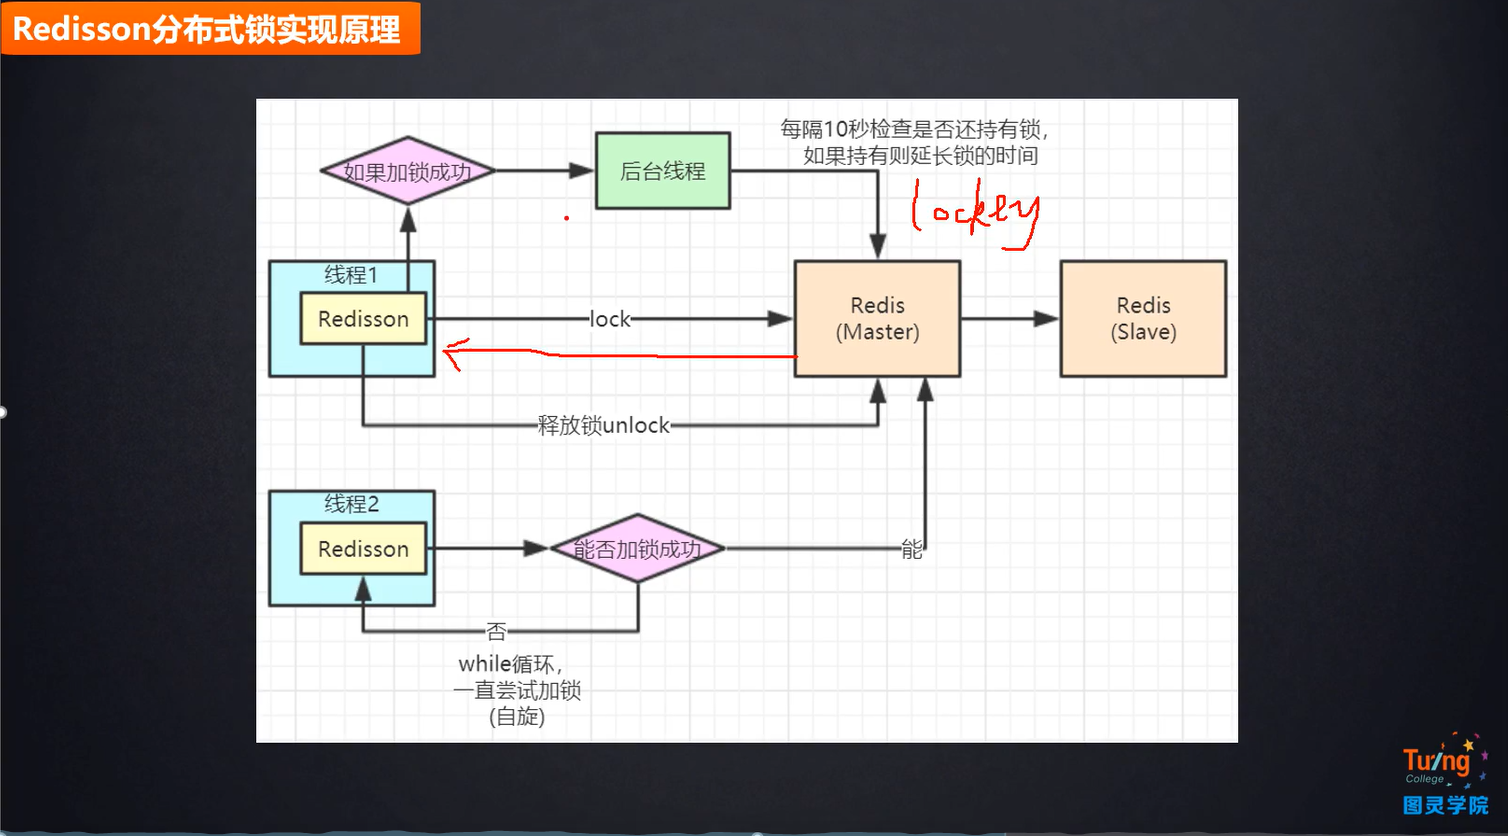
\includegraphics[width=0.7\linewidth]{figures/redission.png}
	\caption{redission}
	\label{fig:redission}
\end{figure}
\subsubsection{如何查看线程死锁}
0. 使用ps H -eo pid,tid,\%cpu|grep 2783 可以查看java进程中的线程
1. 使用jstack命令来查看 \par
2. 对于mysql 使用select * from INFOMATION\_SCHEMA.INNODB\_LOCKS 查看正在锁的事物 \par
3. 查看等待锁的事物 SELECT * FROM INFORMATION\_SCHEMA.INNODB\_LOCK\_WAITS \par
\subsubsection{线程之间如何进行通讯的}
1. 使用共享内存或基于网络来进行通信 \par
2. 如果是通过共享内存来进行通信
\subsubsection{快速失败(fail-fast) 和 安全失败(fail-safe) 的区别是什么?}
\begin{enumerate}
	\item java.util包下面的所有的集合类都是快速失败的, 而java.util.concurrent包下面的所有类都是安全失败的. 快速失败的迭代器会抛出ConcurrentModificationException异常, 而安全失败的迭代去永远不会抛出这样的异常.

\end{enumerate}
\subsubsection{异常}
(1) Throwable(可抛出) 超类, 有两个子类Error 和 exception 错误和异常
\subsubsection{synchronized的底层实现细节}
1. synchronized作用 \par
原子性: synchronized保证语句内操作是原子的 \par
可见性: synchronized保证可见性(通过在执行unlock之前, 必须先报此变量同步回主内存实现) \par
有序性: synchronized保证有序性(通过"一个变量在同一时刻只允许一条线程对其进行lock操作") \par
可见性补充: 	其实真正解决这个问题的是JMM关于Synchronized的两条规定:
\par
1、线程解锁前,必须把共享变量的最新值刷新到主内存中; \par
2、线程加锁时,讲清空工作内存中共享变量的值,从而使用共享变量是需要从主内存中重新读取最新的值(加锁与解锁需要统一把锁) \par
\subsubsection{线程池参数}
ThreadPoolExecutor的创建参数: \par
(1) corePoolSize, 核心运行的线程个数, 若线程池已创建的线程数小于corePoolSize, 即使此时存在空闲线程, 也会通过创建一个新线程来执行该任务. \par
(2) maximumPoolSize: 最大线程个数, 当大于这个值就会将准备新加入的异步任务有一个丢弃处理机制来处理, 大于corePoolSize且小于maxmumPoolSize存入等待队列,\par
(3) workQueue: 任务等待队列, 当达到corePoolSize的时候就向该等待队列放入线程信息.\par
(4) keepAliveTime: 默认0, 当线程没有任务处理后空闲线程保持多长时间, 不推荐使用, 一般会中止超过corePoolSize数量的线程资源, 空闲线程时间超过keepAliveTime, 线程将会被回收 \par
(5) threadFacory: 构造Thread方法, 使用默认的default实现. \par
(6) defaultHandler: 当maximumPoolSize达到后丢弃处理的方法实现, java默认是丢出异常. \par

\subsubsection{你觉得核心线程数和最大线程数之间应该如何设置呢}
1. 对于CPU密集型任务,由于CPU密集型任务的性质,导致CPU的使用率很高,如果线程池中的核心线程数量过多,会增加上下文切换的次数,带来额外的开销。因此,一般情况下线程池的核心线程数量等于CPU核心数+1。

2. 对于I/O密集型任务,由于I/O密集型任务CPU使用率并不和很高,可以让CPU在等待I/O操作的时去处理别的任务,充分利用CPU。因此,一般情况下线程的核心线程数等于2*CPU核心数。


\subsubsection{sychronized和ReentrantLock的区别}
1. sychronized是一个关键字, ReentrantLock是一个类 \par
2. synchronized会自动的加锁和释放锁, ReentrantLock是一个类 \par
3. sychronized的底层是jvm层面的锁, ReentrantLock是API层面的锁 \par
4. sychronized是非公平锁, ReentrantLock可以选择公平锁或非公平锁 \par
5. sychronized锁的是对象, 锁信息保存在对象头中, ReentrantLock锁的是线程 \par
6. sychronized底层有一个锁升级的过程 \par
\subsubsection{线程池ThreadPoolExecutor中使用的BlockQueue}
(1) 直接提交队列: 简单来说使用SynchronousQueue队列,提交的任务不会被保存,总是会马上提交执行。如果用于执行任务的线程数量小于maximumPoolSize,则尝试创建新的进程,如果达到maximumPoolSize设置的最大值,则根据你设置的handler执行拒绝策略。因此这种方式你提交的任务不会被缓存起来,而是会被马上执行,在这种情况下,你需要对你程序的并发量有个准确的评估,才能设置合适的maximumPoolSize数量,否则很容易就会执行拒绝策略;\par
(2) 有界的任务队列可以使用ArrayBlockingQueue实现,若有新的任务需要执行时,线程池会创建新的线程,直到创建的线程数量达到corePoolSize时,则会将新的任务加入到等待队列中。若等待队列已满,即超过ArrayBlockingQueue初始化的容量,则继续创建线程,直到线程数量达到maximumPoolSize设置的最大线程数量,若大于maximumPoolSize,则执行拒绝策略。在这种情况下,线程数量的上限与有界任务队列的状态有直接关系,如果有界队列初始容量较大或者没有达到超负荷的状态,线程数将一直维持在corePoolSize以下,反之当任务队列已满时,则会以maximumPoolSize为最大线程数上限。\par
(3) 使用无界任务队列,LinkedBlockingQueue 实现线程池的任务队列可以无限制的添加新的任务,而线程池创建的最大线程数量就是你corePoolSize设置的数量,也就是说在这种情况下maximumPoolSize这个参数是无效的,哪怕你的任务队列中缓存了很多未执行的任务,当线程池的线程数达到corePoolSize后,就不会再增加了;若后续有新的任务加入,则直接进入队列等待,当使用这种任务队列模式时,一定要注意你任务提交与处理之间的协调与控制,不然会出现队列中的任务由于无法及时处理导致一直增长,直到最后资源耗尽的问题。 \par
(4) 优先任务队列:优先任务队列通过PriorityBlockingQueue实现,
\subsubsection{Executors 工厂类实现线程池}
通过创建不同的ThreadPoolExecutor参数.\par
(1) FixedThreadPool 定长, corePoolSize == maxmumPoolSize   \par
(2) SingleThreadExecutor 单一线程 无界队列 \par
以上两种可能会堆积大量的请求, 从而引起OOM异常 \par
(3) CachedThreadPool 采用maxmumPoolSize为无限大, 容易创建大量线程, 从而耗尽系统资源. \par

submit  基于  Future 来包装返回值对象, 使用callable来进行调用有返回值

execute 基于 runnable 来实现线程池, 没有返回值
\begin{lstlisting}
    final ExecutorService service = Executors.newFixedThreadPool(5);
	Future<String> f = service.submit(new Callable<String>() {
		@Override
		public String call() throws Exception {
			Thread.sleep(3000);
			System.out.println("calld方法执行了");
			return "call方法返回值";
		}
	});
	System.out.println(f.get());
	service.execute(new Runnable() {
		@Override
		public void run() {
			try {
				Thread.sleep(1500);
			} catch (InterruptedException e) {
				e.printStackTrace();
			}
			System.out.println("fdasfdsa");
			return ;
		}
	});
	service.shutdown();
\end{lstlisting}
\subsubsection{线程池的拒绝策略}
(1) abortPolicy 默认: 直接抛出异常 \par
(2) CallerRunsPolicy:  直接调用主线程来执行任务. \par
(3) DiscardPolicy: 不能执行的任务被删除, 和abortPolicy一样, 但是不抛出异常. \par
(4) DiscardOldestPolicy: 位于工作队列头部的任务将被删除, 然后重新执行程序. \par
\subsubsection{8种基本数据类型}
\begin{table}[!htbp]
	\centering
	\caption{实现}
	\begin{tabular}{|l|r|}

		\hline
		类型    & 大小(注释/包装类) \\
		\hline
		byte    & 8(Byte)           \\
		\hline
		short   & 16(Short)         \\
		\hline
		int     & 32(Integer)       \\
		\hline
		long    & 64(Long)          \\
		\hline
		float   & 32(Float)         \\
		\hline
		double  & 64(Double)        \\
		\hline
		char    & 16(Character)     \\
		\hline
		boolean & 8(Boolean)        \\
		\hline
	\end{tabular}
\end{table}
\subsubsection{Comparable \& Comparator 区别}
Comparable 是接口 能力赋予
\begin{lstlisting}
public interface Comparable<T> {
	public int compareTo(T o);
}
\end{lstlisting}
Comparator 是外部比较器, 也是接口, 类似于 C++sort中自定义的cmp函数
\begin{lstlisting}
Collections.sort(list, new Comparator<Person2>() {
	public int compare(Person o1, Person o2) {
		return o1.getAge() - o2.getAge();
	}
})
\end{lstlisting}
\subsubsection{java采用值传递还是引用传递?}
采用值传递, 但是因为采用浅拷贝, 所以会修改传递的对象的相关属性.
\subsubsection{java深拷贝和浅拷贝}
实现了Coneable接口实现深拷贝.
\subsubsection{java"==" 和 equals 的区别}
1. "==" : 如果是基本数据类型, 则直接对值进行比较, 如果是引用数据类型, 则是对他们的地址进行比较;
\par
2. equals方法继承Object类, 在具体实现时可以覆盖父类中的实现. 看一下Object中equals的源码发现, 它的实现也是对\textbf{对象的地址}进行比较, 可以覆盖实现这个方法, 如果两个对象的类型一致, 并且内容一致, 则返回true.
\par
在实际开始中总结:
\par
(1) 类未复写equals, 则使用equals方法比较两个对象时, 相当于==比较, 及两个地址是否相等. 地址相等, 返回true, 地址不相等, 返回false.
\par
(2) 类复写equals方法, 走复写之后的判断方式. 通常, 我们会将equals复写成: 当两个对象内容相同时, 则equals返回true, 内容不同时, 返回false.
\par
对于set, hashMap, hashset等, 还要重写hashCode值, 比如set判断两个元素是否相等的时候, 会判断hashcode和equals都相等, 则认为相等, 不会添加新元素.
\subsubsection{String和StringBuilder, StringBuffer的区别}
String是不可变字符串对象(final的char数组), StringBuilder和StringBuffer(线程安全)是可变字符串对象.
\par
为什么String是final修饰的?
\par
1. 为了实现字符串池, 因为只有当字符串是不可变的, 字符串池才有可能实现.
\subsubsection{Java反射机制}
简单来说就是在, 运行状态中, 对于任意一个类, 都能够知道这个类的所有属性和方法; 对于任意一个对象, 都能够调用它的任意方法和属性; 并且能改变它的属性. 这种动态获取的信息以及动态调用对象的方法的功能称为Java语言的反射机制.
\par
优点: 代码灵活度提高
\par
缺点: 性能瓶颈, 性能较慢.
\subsubsection{简述面向对象三大特征, 继承, 封装, 多态}
1. 封装
\par
简单来说, 就是使用private方法将没有必要暴露的方法和属性进行隐藏.
\par
2. 继承
\par
继承是从已有的类中派生出行的类, 减少代码冗余.
\par
3. 多态
\par
父类引用指向不同子类对象.
\subsubsection{多态}
一般使用instance of 来判断对象的子类关系. 增加向下转型的健壮度. \par
\subsubsection{内部类}
(1) 静态内部类访问外部变量必须是静态的. \par
(2)
\subsubsection{红黑树}
一般考察红黑树: 只考察概念.
\begin{figure}
	\centering
	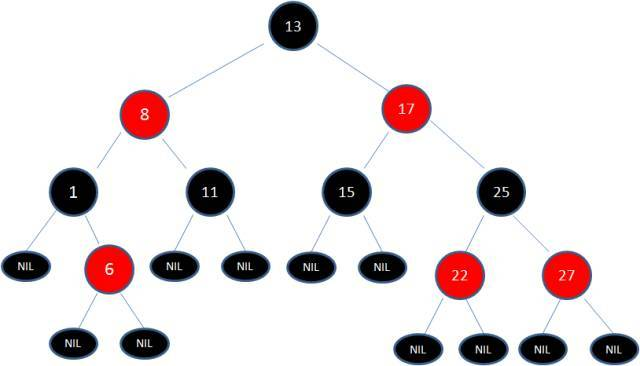
\includegraphics[width=0.7\linewidth]{figures/red_black.jpg}
	\caption{redblack}
	\label{fig:red_black}
\end{figure}
\begin{enumerate}
	\item 节点是红色或黑色
	\item 根节点是黑色
	\item 所有叶子都是黑色(叶子是NIL节点).
	\item 每个红色节点必须有两个黑色节点
	\item 从任一节点到其每个叶子的所有简单路径都包含相同数目的黑色节点.

\end{enumerate}

\subsubsection{hashmap的数据结构}
\begin{enumerate}
	\item jdk1.7 由 数组 + 链表  来构成
	\item jdk1.8 由 数组 + 链表 + 红黑树 来构成
	\item jdk1.8的时候, 当元素不超过64个的时候, 不会出现链表转红黑树, 当元素超过64个的时候, 会出现链表转红黑树.
	\item jdk1.8 当链表长度达到8个的时候, 链表会转为红黑树, 当红黑树元素长度退回到6个的时候会出现红黑树转为链表.
	\item jdk1.7 采用头插法, jdk1.8采用尾插法.
\end{enumerate}
\subsubsection{hashmap的put方法}
1. 根据Key通过哈希算法与与运算得到数组下标 \par
2. 如果数组下标位置元素为空, 则将key和value封装为Entry对象并放入该位置 \par
3. 如果数组下标元素不为空 \par
1.7, 则先判断是否需要扩容, 如果要扩容就进行扩容, 如果不用扩容就生成Entry对象, 并使用头茶法添加到当前位置的链表中 \par
1.8 先判断当前位置上Node的类型, 看是红黑树Node还是链表Node \par
a. 如果是红黑树Node, 则将key和value 封装为一个红黑树节点并添加到红黑树中 \par
b. 如果是链表节点, 使用尾插法插入到链表的最后位置去, 插入完后会判断当街链表的个数看是否需要转为红黑树(超过8个)元素. \par
c. 判断是否需要扩容(0.75*16默认值), 需要扩容就扩容, 不需要就结束PUT方法 \par

JDK8则因为巧妙的设计,性能有了大大的提升:由于数组的容量是以2的幂次方扩容的,那么一个Entity在扩容时,新的位置要么在原位置,要么在原长度+原位置的位置。
\subsubsection{介绍一下ThreadLocal}
1. ThreadLocal 是java中所提供的的线程本地存储机制, 可以利用该机制将数据缓存在某个线程内部, 该线程可以在任意时刻, 任意方法中获取缓存的数据 \par
2. ThreadLocal 底层是通过ThreadLocalMap来实现的, 每个Thread对象中都存在一个ThreadLocalMap, Map的key为ThreadLoacl对象, Map的value为需要缓存的值 \par
3. 如果在线程池中使用ThreadLocal会造成内存泄露, 因为当ThreadLocal对象使用完后, 应该要报设置的key, value 也就是Entry对象进行回收, 但线程池中的线程不会回收, 而线程对象是通过强引用指向ThreadLocalMap, ThreadLocalMap也是通过强引用指向Entry对象, 线程不被回收, Entry对象也就不会被回收, 从而出现内存泄露, 解决方法是, 在使用了ThreadLocal对象之后, 手动调用ThreadLocal的remove方法, 手动清除Entry对象. \par
\subsubsection{heap和stack有什么区别}
\begin{enumerate}
	\item java的内存分为两类, 一类是堆内存, 一类是栈内存
	\item 栈内存是指程序进入一个方法时, 会为这个方法单独分配一块私属存储空间, 用于存储这个方法内部的局部变量. 当这个方法结束时, 分配给这个方法的栈会释放, 这个栈中的变量也随之释放.
	\item 使用new创建的对象存放在堆里, 不会随方法的结束二小时. 方法中的局部变量使用final修饰后, 放在堆中, 而不是栈中.

\end{enumerate}

\subsubsection{Array 和 ArrayList 的区别}
\begin{enumerate}
	\item Array 大小固定(int a[]={1,2,3}), ArrayList 大小是动态变化的.
\end{enumerate}
transient: 将不需要序列化的属性前添加关键字transient,序列化对象的时候,这个属性就不会被序列化。

默认初始化大小是10个容量.

$$int newCapacity = oldCapacity + (oldCapacity >> 1);$$

新的大小是旧的大小的1.5倍. 扩容会调用Arrays.copyOf操作, 然后申请新的大小.
\subsubsection{Java各种锁: 悲观锁, 泪管所, 自旋锁, 偏向锁, 轻量/重量锁, 读写锁, 可重入锁}
悲观锁和乐观锁指的是并发情况下的两种不同策略, 是一种宏观的描述.
\par

\begin{enumerate}
	\item 悲观锁和乐观锁指的是并发情况下的两种不同策略, 是一种宏观的描述.

\end{enumerate}
\subsubsection{Collection 和 Collections 的区别}
\begin{enumerate}
	\item Collection 是集合类的上级接口, 继承他的接口主要是set和list
	\item Collections 类数针对集合类的一个帮助类. 它提供了一系列的静态方法对各种集合的搜索, 排序, 线程安全化等操作.
\end{enumerate}
\subsubsection{接口与抽象类区别}
\begin{enumerate}
	\item 类可以实现多个接口但只能继承一个抽象类
	\item 接口中变量被隐性制定为public static final, 方法被指定为 public abstract
	\item 接口里面所有的方法都是Public的, 抽象类允许Private, Protected方法
	\item JDK接口可以实现默认方法和静态方法, 前面加defalut, static关键字.
	\item 设计层面: 抽象类是对事物的抽象, 接口是对行为的抽象.
\end{enumerate}
\begin{lstlisting}
public interface InterfaceJDK8 {
	
	/*接口的普通抽象方法*/
	public void common(String str);
	
	/*jdk1.8 默认方法:
	允许在已有的接口中添加新方法,而同时又保持了与旧版本代码的兼容性,
	默认方法与抽象方法不同之处在于抽象方法必须要求实现,但是默认方法则没有要求实现,
	相反,接口提供了一个默认实现,这样所有的接口实现者将会默认继承他
	(如果有必要的话,可以覆盖这个默认实现)。
	接口的默认方法:得到接口的实现类对象,直接用对象的引用.方法名。默认方法可以被实现类覆盖。
	*/
	default public void defaultMethod(String str){
		System.out.println("InterfaceJDK8:" + str);
	}
	
	/*jdk1.8 静态方法:
	允许在已有的接口中添加静态方法,接口的静态方法属于接口本身,不被继承,也需要提供方法的现。
	*/
	public static void staticMethod(String str){
		System.out.println("InterfaceJDK8:" + str);
	}
	
}
\end{lstlisting}
\subsubsection{ArrayList和LinkedList内部实现大致是怎样的? 他们之间的区别和优缺点}
\begin{enumerate}
	\item ArrayList: 内部使用数组的形式实现了存储, 利用数组的小表进行元素的访问, 因此对元素的随机访问速度非常快. 初始化大小为10, 插入新元素的时候, 会判断是否需要扩容, 扩容的步长是0.5倍原容量, 扩容方式是利用数组的复制, 因此有一定的开销
	\item LinkedList:内部使用双向链表的结构实现存储, LinkedList有一个内部类作为存放元素的单元, 里面有三个属性, 用来存放元素本身以及前后2个单元的引用, 另外LinkedList内部还有一个Header属性, 用来标识起始位置, LinkedList的第一个单元和最后一个单元都会指向header, 因此形成了一个双向链表结构.
	\item LinkedList还额外实现了Deque接口, 所以LinkedList还可以当做队列来使用. \par
\end{enumerate}
\subsubsection{==和equals的区别}
==是运算符, 而equals是Object的基本方法, ==用于基本数据的类型比较, 或者是比较两个对象的引用是否相同, equals用于比较两个对象的值是否相等, 例如字符串的比较.
\subsubsection{hashCode方法的作用}
\begin{enumerate}
	\item 如果两个对象equals方法相等, 那么hashCode一定相同
	\item 如果两个对象的hashCode相同, 并不表示两个对象相同(只能表示hash碰撞相同), equals方法相同.
\end{enumerate}
\subsubsection{反射}
简单来说, 在运行状态中, 对于任意一个类, 都能够知道这个类的所有属性和方法, 对于任意一个对象, 都能够调用他的任意方法和属性, 并且能够改变他的属性.
\subsubsection{简述Java内存模型(JMM)}
简单来说就是, java中存在一个主内存, java中所有变量都存在主内存中, 对所有线程进行共享, 而每个线程又存在自己工作内存, 工作内存存储的是主存中某些变量的拷贝, 线程对所有变量的操作并非发生在主存区, 而是发生在工作内存中, 线程之间是不能直接相互访问, 变量在程序中的传递主要依赖主存完成.  \par
\begin{figure}
	\centering
	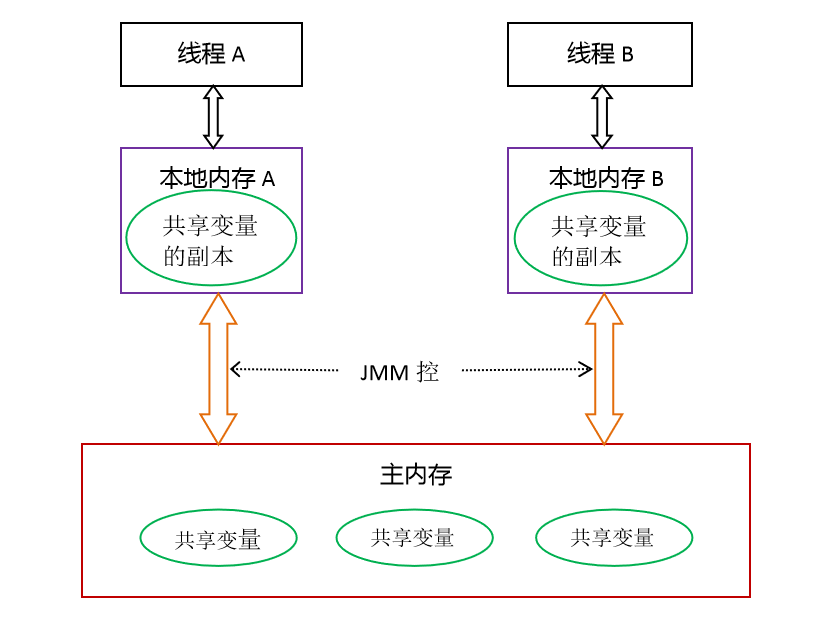
\includegraphics[width=0.7\linewidth]{figures/JMM.png}
	\caption{JMM}
	\label{fig:JMM}
\end{figure}
\subsubsection{Java内存模型中的可见性, 原子性和有序性}
可见性, volatile \par
原子性, 各种锁 \par
有序性, 线程内有序 \par
\subsubsection{happen-before原则}
虽然有好几个, 但基本上描述模糊的就不写了\par
(1) 锁的happen-before, 就是同一个锁的unlock操作happen-before此锁的lock操作. \par
(2) 传递性: A hb b, b hb c; A happen-before C; \par
(3) 对象的构造函数在finalize方法之前.
\subsubsection{wait/notify, await/singal}
Condition 的 await,signal, singalAll 与 Object 的 wait, notify, notifyAll 都可以实现的需求,两者在使用上也是非常类似,都需要先获取某个锁之后才能调用,而不同的是 Object wait,notify 对应的是 synchronized 方式的锁,Condition await,singal 则对应的是 ReentrantLock (实现 Lock 接口的锁对象)对应的锁 \par
下方是Condition的示例
\subsubsection{多线程wait和sleep区别}
(1) 主要在获得执行权和释放锁之间的区别, wait会释放执行权, 然后释放锁 , sleep 只会释放执行权 \par
(2) 如果notifyAll() 如果有多个线程在等待, 只会有一个线程获得执行权. \par
\subsubsection{Collection<? extends Person> s}
这叫泛型上限, 这样取出都是按照上限类型来运算的. 不会出现安全隐患
\begin{lstlisting}
public class Message {
	/** 当前消息数量*/
	private int count = 0;
	/** 信息存放最大限数*/
	private int maximum = 20;
	/** 重入锁*/
	private Lock lock;
	/** 生产者锁控制器*/
	private Condition producerCondition;
	/** 消费者锁控制器*/
	private Condition consumerCondition;
	
	public Message() {}
	
	public Message(final Lock lock, final Condition producerCondition, final Condition consumerCondition) {
		this.lock = lock;
		this.producerCondition = producerCondition;
		this.consumerCondition = consumerCondition;
	}
	
	/**
	* 生产消息
	* */
	public void set() {
		/** 获取锁*/
		lock.lock();
		try {
			if (count <= maximum) {
				/** 生产一个消息*/
				System.out.println("生产者 线程" + Thread.currentThread().getName() + "生产了一个消息, 当前有" + (++count) + "个消息");
				/** 唤醒等待的消费者*/
				consumerCondition.signal();
			} else {
				try {
					/**
					* 如果当前消息大于 maximum信息最大数
					* 生产者进入睡眠/等待状态
					* */
					producerCondition.await();
					System.out.println("生产者 线程" + Thread.currentThread().getName() + "进入睡眠");
				} catch (InterruptedException e) {
					e.printStackTrace();
				}
			}
		} finally {
			/** 释放锁*/
			lock.unlock();
		}
	}
	
	/**
	* 消费消息
	* */
	public void get() {
		/** 获取锁*/
		lock.lock();
		try {
			if (count > 0) {
				/** 消费一个消息*/
				System.out.println("消费者 线程" + Thread.currentThread().getName() + "消费了一个消息, 当前有" + (--count) + "个消息");
				/** 唤醒等待的生产者*/
				producerCondition.signal();
			} else {
				try {
					/** 如果没有消息, 消费者进入睡眠/等待状态*/
					consumerCondition.await();
					System.out.println("消费者 线程" + Thread.currentThread().getName() + "进入睡眠");
				} catch (InterruptedException e) {
					e.printStackTrace();
				}
			}
		} finally {
			/** 释放锁*/
			lock.unlock();
		}
	}
	
}

public class Producer implements Runnable {
	private Message message;
	public Producer(Message message) {
		this.message = message;
	}
	
	@Override
	public void run() {
		while(true) {
			try {
				Thread.sleep(500);
			} catch (InterruptedException e) {
				e.printStackTrace();
			}
			message.set();
		}
	}
	
}
public class Consumer implements Runnable {
	private Message message;
	public Consumer(Message message) {
		this.message = message;
	}
	
	@Override
	public void run() {
		while(true) {
			try {
				Thread.sleep(1000);
			} catch (InterruptedException e) {
				e.printStackTrace();
			}
			message.get();
		}
	}
	
}
import java.util.concurrent.locks.Condition;
import java.util.concurrent.locks.Lock;
import java.util.concurrent.locks.ReentrantLock;

public class App {
	public static void main(String[] args) {
		/** 重入锁*/
		final Lock lock = new ReentrantLock();
		/** 生产者锁控制器*/
		final Condition producerCondition = lock.newCondition();
		/** 消费者锁控制器*/
		final Condition consumerCondition = lock.newCondition();
		final Message message = new Message(lock, producerCondition, consumerCondition);
		/** 建几个生产线程*/
		new Thread(new Producer(message)).start();
		new Thread(new Producer(message)).start();
		new Thread(new Producer(message)).start();
		/** 建几个消费线程*/
		new Thread(new Consumer(message)).start();
		new Thread(new Consumer(message)).start();
		new Thread(new Consumer(message)).start();
		new Thread(new Consumer(message)).start();
	}
	
}


\end{lstlisting}
\subsubsection{线程的状态有哪些?}
(1) 新建状态(NEW): 线程创建之后 \par
(2) 可运行(RUNNING): 可能正在运行, 也可能正在等待时间片 \par
(3) 阻塞(BLOCKED): 等待获取一个排它锁, 如果期限陈释放了锁就会结束此状态. \par
(4) 无线等待(WAITING): 等待其他线程显式地唤醒, 否则不会被分配CPU时间片片 \par
(5) 限期等待(TIME\_WAITING): 如果没人唤醒在一定时间内系统会自动唤醒 \par
(6) 终止(TERMINATED): 可以是线程结束任务之后自己结束, 或者产生了异常而结束 \par
线程创建之后处于New状态, 调用start()方法后开始运行, 线程这时候处于Ready可运行状态. 可运行状态的线程获得cpu时间片后就处于RUNNING状态. 当线程执行wait()方法之后, 线程进入WAITING(等待)状态. 进入等待状态的线程需要依靠其他线程的通知才能够返回到运行状态, 而TIME\_WAITING超时等待状态相当于在等待状态的基础上增加了超时限制, 比如通过SLEEP方法或wait放假将java线程至于TIME\_WAITING状态, 到超时之后, java线程将会发挥RUNNABLE状态. 当线程调用同步方法是,在没有获取到所的情况下,线程将会进入到BLOCK状态. 执行完Runnable的run()方法之后将会进入到TERMINATED状态.
\begin{figure}
	\centering
	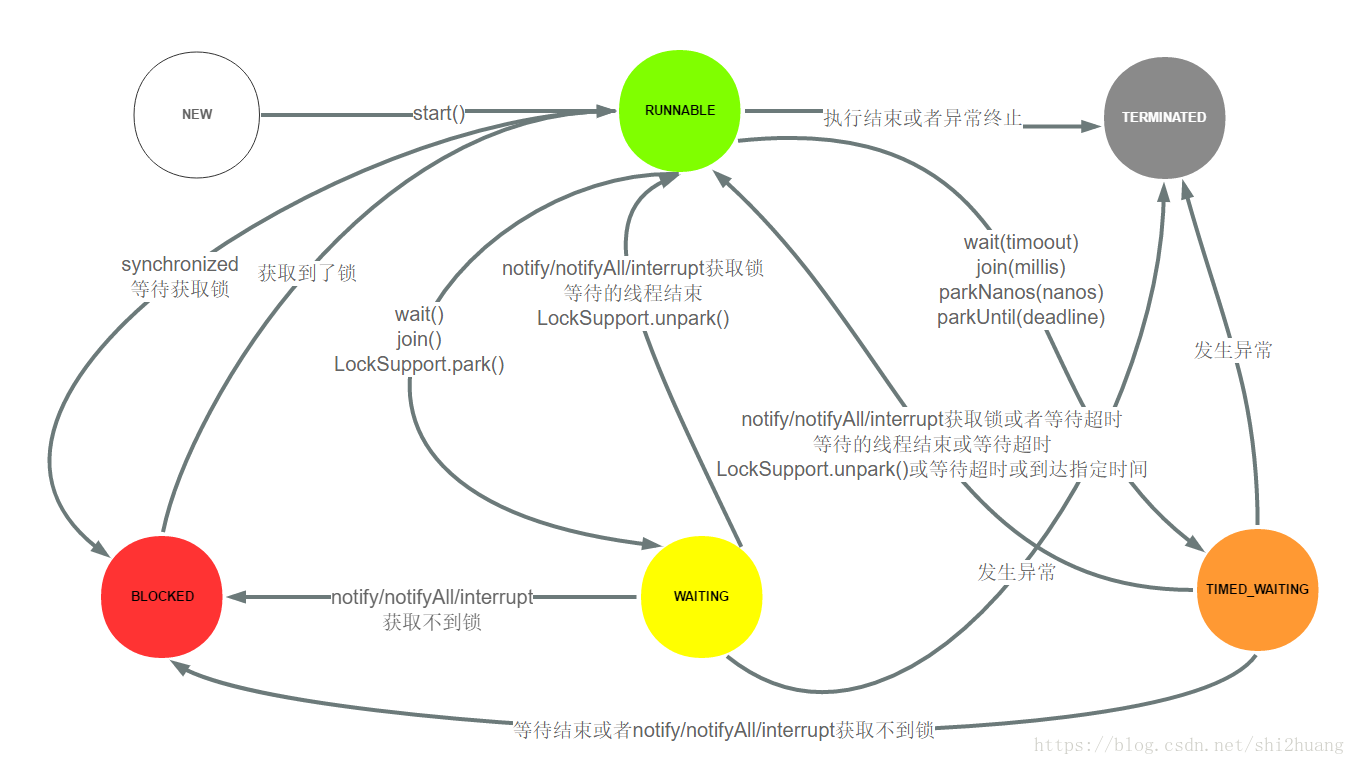
\includegraphics[width=0.7\linewidth]{figures/javaThreadState.png}
	\caption{javaThreadState}
	\label{fig:javaThreadState}
\end{figure}
\subsubsection{进程的状态有哪些?}
就绪状态: 已获除CPU以外所需的资源, 等待分配处理机资源

运行状态: 占用处理机资源运行

阻塞状态: 进程等待某种条件,在满足之前无法执行


new 行启动进程获除CPU以外的资源被准许(admitted)进入就绪状态ready, 就绪进程获得系统分配CPU资源后背调度器调度(scheduler dispatch)进入运行太running, 运行态进程在执行完任务后退出(exit)进程终止terminated.

运行太进程当时间片用完时候会先中断(interrupt) 进入到就绪状态, 等待下次时间片轮转分配CPU资源. 运行太进程当遇到等待用户输入或时间等待(IO or event wait) 会进入阻塞态waiting, 阻塞态进程IO输入完毕或时间完成(IO or event completion) 会进入到就绪太等待系统分配CPU资源.

\begin{figure}
	\centering
	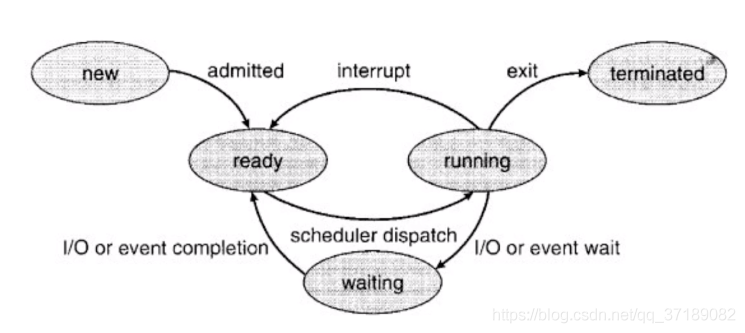
\includegraphics[width=0.7\linewidth]{figures/processorstatus.png}
	\caption{processorstatus}
	\label{fig:processorstatus}
\end{figure}

\subsubsection{创建线程的几种方式}
(1) 继承Thread类创建线程 \par
定义Thread类的子类, 并重写该类的run方法\par
创建实例\par
调用实例start()方法 \par
(2) 实现Runnable接口创建线程 \par
实现一个接口类, 重新run方法. \par
创建Runnable实现类实例, 并以此实例作为Thread的target来创建Thread对象, 该Thread对象才是真正的线程对象. \par
调用线程对象start方法来启动该线程\par
(3) 使用Callable和Future创建线程: 与Runnable相比Callable是有返回值的, 返回值通过FutureTask进行封装 \par
创建Callable接口的实现类, 并实现call()方法, 该call()方法将作为线程执行体, 兵器有返回值 \par
创建Callbale实现类实例, 使用FutureTask类来包装Callable对象, 该FutureTask对象封装了该Callable对象的call()方法的返回值. \par
使用FutureTask对象作为Thread对象的target创建biang启动新线程\par
调用FutureTask对象的get()方法来获得子线程执行结束后的返回值 \par
(4) 使用线程池例如Executor框架(工厂方法) \par
(5) 创建线程的方式的对比\par
1. Runnable 不可以抛出异常, Callable可以 \par
2. Runnable 不可以有返回值, Callable 通过封装FutureTask 可以拿到返回值 \par
\subsubsection{synchronized锁升级: 无锁, 偏向锁, 轻量级锁, 重量级锁(与锁的优化一起学习}
这个叫做锁的膨胀. \par
(1) 偏向锁, 初次执行到synchronized代码块的时候, 锁对象变成偏向锁, 通过CAS修改对象投里的锁标志位, 字面意思是"偏向于第一个获得它的线程"的锁. 会存储获取锁的线程的地址. 偏向锁解锁, 不需要修改对象头的markword, 减少了一次CAS操作, 锁不会释放, 但是遇到冲突, 会由JVM来进行判断升级. 执行完同步代码块之后, 线程并不会主动释放偏向锁, 当第二次达到同步代码块时, 线程会判断此时持有锁的线程是否就是自己(持有锁的线程ID也在对象头里), 如果是正常往下执行. 由于之前没有释放锁, 这里也就不需要重新加锁. 如果自始至终使用锁的线程只有一个, 很明显偏向锁几乎没有额外开销, 性能极高. \par
(2) 轻量级锁, 自旋锁, 地担忧第二个线程加入锁竞争, 偏向锁, 就升级为轻量级锁. 只有当某线程获取锁的时候, 发现该锁已经被占用, 只能等待其实方, 这才发生了锁的竞争. 在所竞争下, 没有抢到锁的线程将自旋, 即不停的循环判断锁是否能够被成功获取. 长时间的自选操作是非常消耗资源的, 一个线程持有锁, 其他线程就只能在原地空号CPU. 如果达到某个最大自旋次数, 会将轻量级锁升级为重量级锁. 当后续线程尝试获取锁时, 直接将自己挂起.\par
(3) 偏向锁, 假定条件只有一个线程去获取锁 \par
(4) 轻量级锁, 假定条件是 多个线程交替去获取锁 \par
\subsubsection{如何使用synchronized}
1. 普通同步方法
